\chapter{Einleitung}
\label{chap:einleitung}
In einer globalisierten und dynamischen Wirtschaftswelt sind Unternehmen zunehmend auf Projekte angewiesen, um ihre Ziele zu erreichen und Wettbewerbsvorteile zu erlangen. Die Personalbeschaffung für solche Projekte erfordert oft spezialisiertes Fachwissen und vielfältige Fähigkeiten, um erfolgreich umgesetzt zu werden. Es ist entscheidend für den Projekterfolg, dass die Personalbeschaffung die passenden Mitarbeiter für ausgewählte Projekte findet. Hier setzt die Entwicklung eines Recommender Systems zur Mitarbeiterempfehlung an. Ein solches System kann Unternehmen dabei unterstützen, den Prozess der Mitarbeiterrekrutierung und -auswahl zu optimieren. Durch die Berücksichtigung verschiedener Kriterien wie Qualifikationen, Fähigkeiten und Erfahrungen kann das Recommender-System dazu beitragen, die Auswahl effektiv zu filtern und diejenigen herauszufiltern, die am besten zu einem Projekt im Unternehmen passen. Ein solches System bietet außerdem den Vorteil, den Prozess der Mitarbeiterempfehlung zu automatisieren und zu beschleunigen. Dies ermöglicht Unternehmen, schneller auf offene Stellen zu reagieren und potenzielle Kandidaten zeitnah zu identifizieren. Dadurch wird die Effizienz der Mitarbeitersuche verbessert und die Qualität der Einstellungsentscheidungen erhöht.\\

Das Potenzial von Recommender Systems wurde auch bei \emph{adesso} entdeckt und nun wird nach und nach Wege gesucht, KI-gestützte Systeme in die eigenen Prozesse zu integrieren. Im internen Projekt \emph{adesso Staffing Advisor} wird an einem Recommender-System zur Mitarbeiterempfehlung für ausgewählte Projekte gearbeitet. Die Umsetzung der Recommender Systems bedient sich verschiedener KI-basierten Ansätze. Als IT-Dienstleister wird \emph{adesso} von Kunden unter anderem mit der Entwicklung individueller Softwarelösungen beauftragt. Derzeit verbringen Führungskräfte jedoch viel Zeit damit, interne Mitarbeiterinnen und Mitarbeiter manuell für Kundenprojekte zu suchen und diese dann aufgrund ihrer Erfahrungen und Fähigkeiten auszuwählen und entsprechend einzusetzen. Ein ganz entscheidender Schritt im Prozess der Mitarbeiterempfehlung ist die Vorverarbeitung der \emph{Bedarfsmeldungen}. Diese beinhalten Informationen zu Projekten und sind eine wertvolle Informationsquelle, die Führungskräften helfen kann, die Empfehlungen effizienter zu gestalten, um dadurch wettbewerbsfähig zu bleiben. Allerdings sind diese oft umfangreich, unsortiert und komplex, was ihre effektive Nutzung erschwert. Dieser Prozess soll durch eine KI-Lösung unterstützt werden. Da es sich bei der Personalsuche um einen geschäftskritischen Prozess handelt, ist der Spielraum für Fehler gering. Im internen Projekt \emph{adesso Staffing Advisor} wird eine durch Large Language Model-gestützte Anwendung entwickelt, die Führungskräfte bei der Suche nach geeignetem Personal für ausgewählte Projekte unterstützt. Der Ansatz des Large Language Modeling ist jedoch nicht deterministisch. Es besteht die Gefahr, dass bei gleichem Input unterschiedliche Ergebnisse erzielt werden. Somit versucht \emph{adesso} durch den Einsatz von Methoden und Technologien neben dem Large Language Model-Ansatz deterministische Ergebnisse zu erzielen, die auf einem ähnlichen Niveau liegen. Ein Ansatz ist die Anwendung von effizienten Methoden und Techniken des Information Retrieval, um so relevante Informationen schnell und präzise aus \emph{Bedarfsmeldungen} zu extrahieren. Die Extraktion wichtiger Schlüsselwörter, Phrasen und Themen ermöglicht es einen besseren Einblick in die Ziele, Methoden und Ergebnisse der Projekte zu bekommen. Dadurch können fundierte Entscheidungen bezüglich der Personalbesetzung getroffen und Ressourcen effizient genutzt werden.\\
\section{Problemstellung}
\label{sec:problemstellung}
Der Staffing-Prozess kann ausschließlich von ausgewählten Mitarbeitenden von adesso durchgeführt werden. Um das Entlastungspotenzial für Führungskräfte durch das Gesamtsystem eines Recommender Systems für Mitarbeiterempfehlungen zu realisieren, ist eine technische Abbildung des Prozesses erforderlich. Dazu sind mehrere Schritte notwendig.
\begin{figure}[H]
	\centering  
	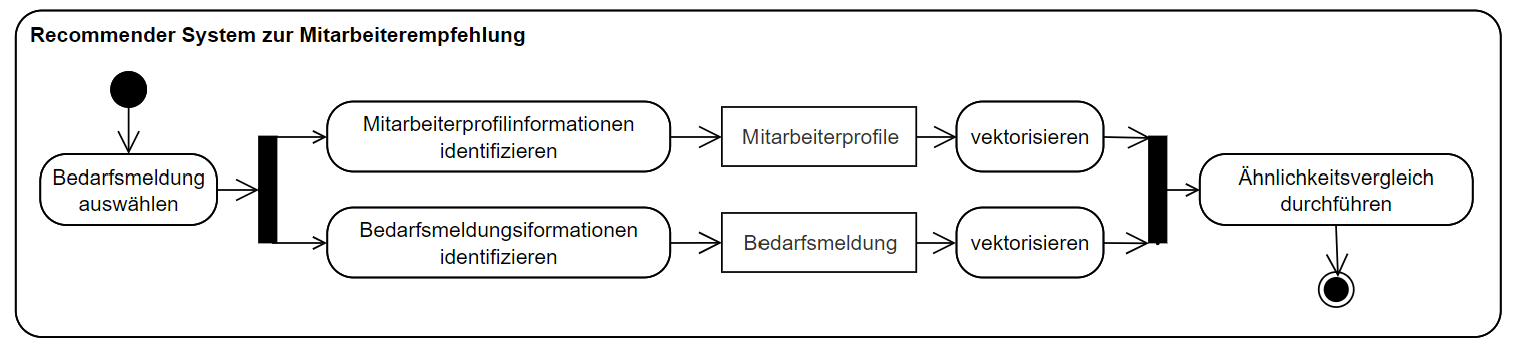
\includegraphics[width=\linewidth]{Abbildungen/recommendersystem.png}
	\caption{Prozess des Recommender System zur Mitarbeiterempfehlung.}
	\label{fig:recommendersystem}
\end{figure}\mbox{} \\
Diese Schritte sind abstrakt als UML-Aktivitätsdiagramm in der Abbildung \ref{fig:recommendersystem} dargestellt. Eine Informationsgewinnung aus den unstrukturierten Projekt- und Mitarbeiterdaten ist unerlässlich, um schließlich den Ähnlichkeitsvergleich für die Empfehlungen durchführen zu können. Diese Ausarbeitung befasst sich mit dem Schritt der Strukturierung und Informationsextraktion der \emph{Bedarfsmeldungen}. Somit steht \emph{adesso} vor der Herausforderung, relevante Informationen effizient aus umfangreichen \emph{Bedarfsmeldungen} zu extrahieren. Obwohl diese Beschreibungen wichtige Einblicke in Ziele, Methoden und Ergebnisse liefern, können sie aufgrund ihres Umfangs und ihrer Komplexität schwer durchsuchbar und analysierbar sein. Die manuelle Identifizierung und Extraktion relevanter Inhalte ist zeitaufwendig und fehleranfällig. Daher stellt sich die Problemstellung: \\

Wie können wir effektive Methoden und Techniken des Information Retrieval und Data-Mining nutzen, um automatisiert relevante Inhalte aus \emph{Bedarfsmeldungen} im spezifischen Kontext der Software Entwicklung zu extrahieren und somit die Effizienz, Genauigkeit und Geschwindigkeit der Informationsgewinnung für Führungskräfte zu verbessern.\\

In der Vergangenheit wurden bereits Methoden im Bereich des automatisierten Recruitings untersucht. Im Projektgeschäft sehen wir uns mit einem Problem konfrontiert, dessen Umfang jedoch präziser definiert werden kann, da die Kandidatenauswahl einem begrenzten Pool unterliegt. Besondere Relevanz hat hierbei die Erstellung einer Standardisierung der \emph{Bedarfsmeldung}, da diese häufig unstrukturiert und mit fehlenden Informationen vorliegt.
\section{Ziele und Ergebnisse der Arbeit}
\label{sec:zieleundergebnis}
Diese Ausarbeitung präsentiert eine umfassende Untersuchung zur Entwicklung eines automatisierten Systems zur Extraktion relevanter Inhalte aus \emph{Bedarfsmeldungen} im Software-Entwicklungs-Kontext.
\begin{itemize}
	\item In der Ausarbeitung wird zunächst ein Konzept einer standardisierten \emph{Bedarfsmeldung} erarbeitet. Dazu wird eine klare Erwartungshaltung hinsichtlich der Anforderungen und Bedürfnisse der Stakeholder entwickeln. Hierfür werden Interviews mit Führungskräften durchgeführt, um die Erwartungen bezüglich einer \glqq{}perfekten\grqq{} \emph{Bedarfsmeldung} herauszuarbeiten. Dieses Konzept dient als Grundlage für die weiteren Entwicklungs- und Evaluierungsphasen.
	\item Es wird an einer ausführbaren prototypischen Software gearbeitet, die \emph{Bedarfsmeldungen} effizient verarbeitet und wichtige Informationen extrahiert. Hierfür wird eine Pipeline in Python aufgebaut und strukturell durch ein Use-Case- und Flussdiagramm dokumentiert. Es werden Modelle des Information Retrieval und Data-Mining implementiert die dazu beitragen, eine \emph{Bedarfsmeldung} in die vorher definierte Struktur umzuformen. Dabei erfolgt zunächst eine eingehende Analyse der Techniken \emph{TF-IDF}, \emph{Text-Ranking-Algorithmen}, \emph{N-Gramm}, \emph{Named Entity Recognition} und Hybride Ansätze, um die besten Ansätze zur Extraktion relevanter Inhalte zu identifizieren. Diese Analyse bildet die Grundlage für die Konzeptionierung des Software-Prototypen, das eine Kombination der erforschten Ergebnisse darstellt.
	\item Um die Leistungsfähigkeit des entwickelten Systems zu evaluieren, werden Testfälle für reale \emph{Bedarfsmeldungen} definiert. Dabei wird überprüft, inwieweit das Ergebnis den Erwartungen entspricht. Mit Hilfe einer manuellen Überprüfung werden Abweichungen, Ähnlichkeiten und Anpassungen analysiert, um Erkenntnisse über die inhaltliche Leistung des Systems und die Techniken zu gewinnen, die allein oder in Kombination mit mehreren Ansätzen die wichtigsten Informationen aus den semi-strukturierten \emph{Bedarfsmeldungen} herausfiltern. Da die Dauer eine entscheidende Rolle spielt, werden auch Zeit und Leistung gemessen. %Diese Ergebnisse werden mit einem neuen Vorverarbeitungsansatz verglichen, der auf dem Large Language Model basiert. Die Performance, Zeit und Ergebnisqualität des entwickelten Systems soll im Vergleich mit diesem alternativen Ansatz die Stärken und Schwächen des entwickelten Systems aufzeigen, um daraus gegebenenfalls weitere Verbesserungsmöglichkeiten zu identifizieren.
\end{itemize}
\section{Aufbau der Arbeit}
\todo{Anpassen}\\

\textbf{Kapitel \ref{chap:einleitung} \nameref{chap:einleitung}} befasst sich mit der Problemstellung und die Zielsetzung der Ausarbeitung. Dazu wird der Aufbau der Arbeit erläutert.\\

\textbf{Kapitel \ref{chap:grundlagen} \nameref{chap:grundlagen}} befasst sich mit grundlegenden Begrifflichkeiten und der Historie von Recommender Systems zum besseren Verständnis der weiteren Kapitel. \\

In \textbf{Kapitel \ref{chap:erwartungshaltung} \nameref{chap:erwartungshaltung}} werden Experteninterviews durchgeführt und analysiert, um eine standardisierte \emph{Bedarfsmeldung} zu entwickeln. \\

\textbf{Kapitel \ref{sec:literaturueberblick} \nameref{sec:literaturueberblick}} wird Literatur zu Methodiken und Ansätze für die Nutzung von Extraktionsmechanismen von Schlüsselwörtern analysiert. \\

In \textbf{Kapitel \ref{chap:implementierung} \nameref{chap:implementierung}} wird auf Basis der erforschten Ergebnisse aus Kapitel \ref{chap:erwartungshaltung} und \ref{sec:literaturueberblick} ein System zur Strukturierung von \emph{Bedarfsmeldungen} entwickelt. \\

In \textbf{Kapitel \ref{chap:evaluation} \nameref{chap:evaluation}} wird das in Kapitel \ref{chap:implementierung} entwickelte System evaluiert. \\

Das abschließende \textbf{Kapitel \ref{chap:ergebnisseausblick} \nameref{chap:ergebnisseausblick}} fasst die wichtigsten Ergebnisse zusammen und gibt einen Ausblick auf mögliche weiterführende Forschungen und Anpassungsmöglichkeiten des entwickelten Systems. \\
\newpage
